
\documentclass[12pt]{amsart}
\usepackage[utf8]{inputenc}
\usepackage{graphicx}
\graphicspath{ {images/} }
\usepackage{float}

\usepackage[swedish]{babel}
\usepackage{geometry} % see geometry.pdf on how to lay out the page. There's lots.
\geometry{a4paper} % or letter or a5paper or ... etc
% \geometry{landscape} % rotated page geometry

% See the ``Article customise'' template for come common customisations

\title{Användarmanual - Operationsförberedelser}
%\author{Daniel Falk}
\date{} % delete this line to display the current date

%%% BEGIN DOCUMENT
\begin{document}

\maketitle
\tableofcontents

\section{Skapa Handbok}
Välj alternativet 'Skapa Handbok' i adminmenyn (se figur \ref{fig:skapa_handbok_meny}).

\begin{figure}[H]
	\begin{center}
	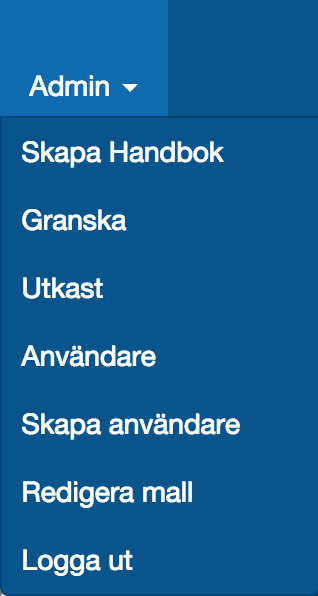
\includegraphics[scale=0.4]{skapa_handbok_meny.png}
	\caption{Skapa handbok meny}
	\label{fig:skapa_handbok_meny}
	\end{center}
\end{figure}

I figur \ref{fig:skapa_handbok} visas vyn för att skapa en ny handbok. Här anger man namn och handbokens specialitet. Tryck skapa handbok för att komma till redigeringsvyn. 
 \begin{figure}[H]
	\begin{center}
	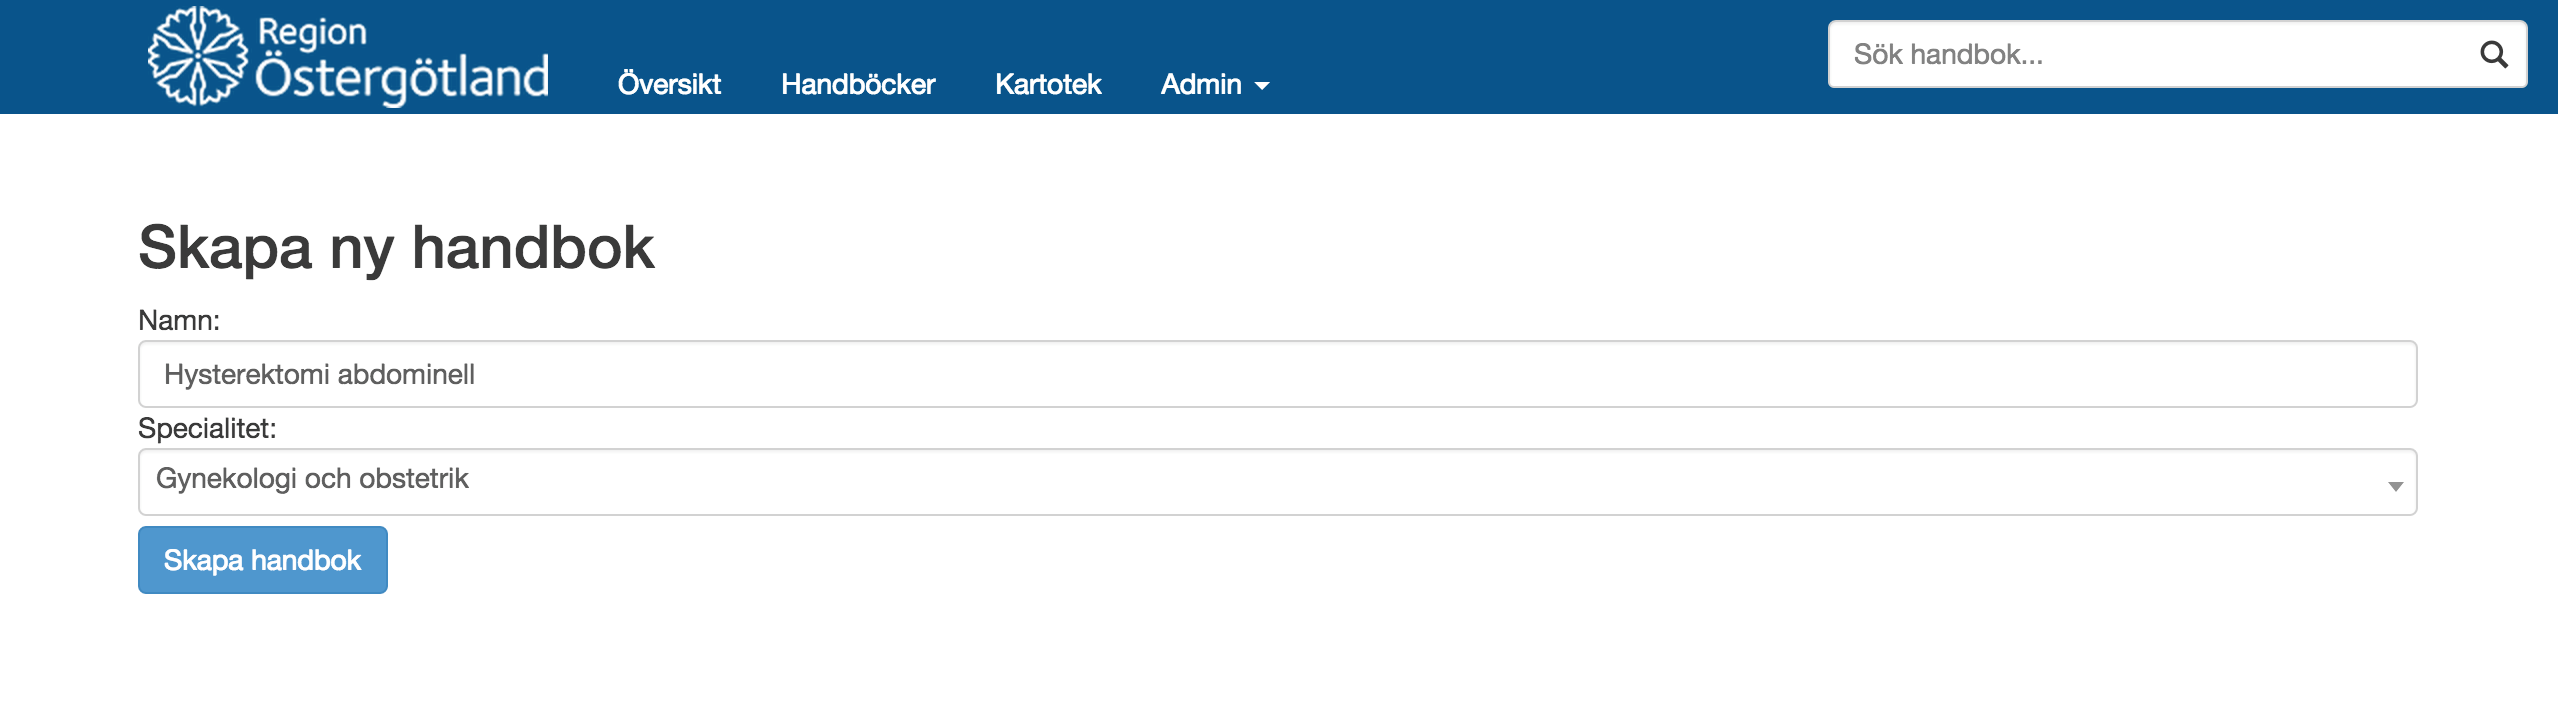
\includegraphics[scale=0.3]{skapa_handbok.png}
	\caption{Skapa handbok}
	\label{fig:skapa_handbok}
	\end{center}
\end{figure}
 
 \section{Redigera Handbok}
Figur \ref{fig:redigeringsvy} visar redigeringsvyn.

  \begin{figure}[H]
	\begin{center}
	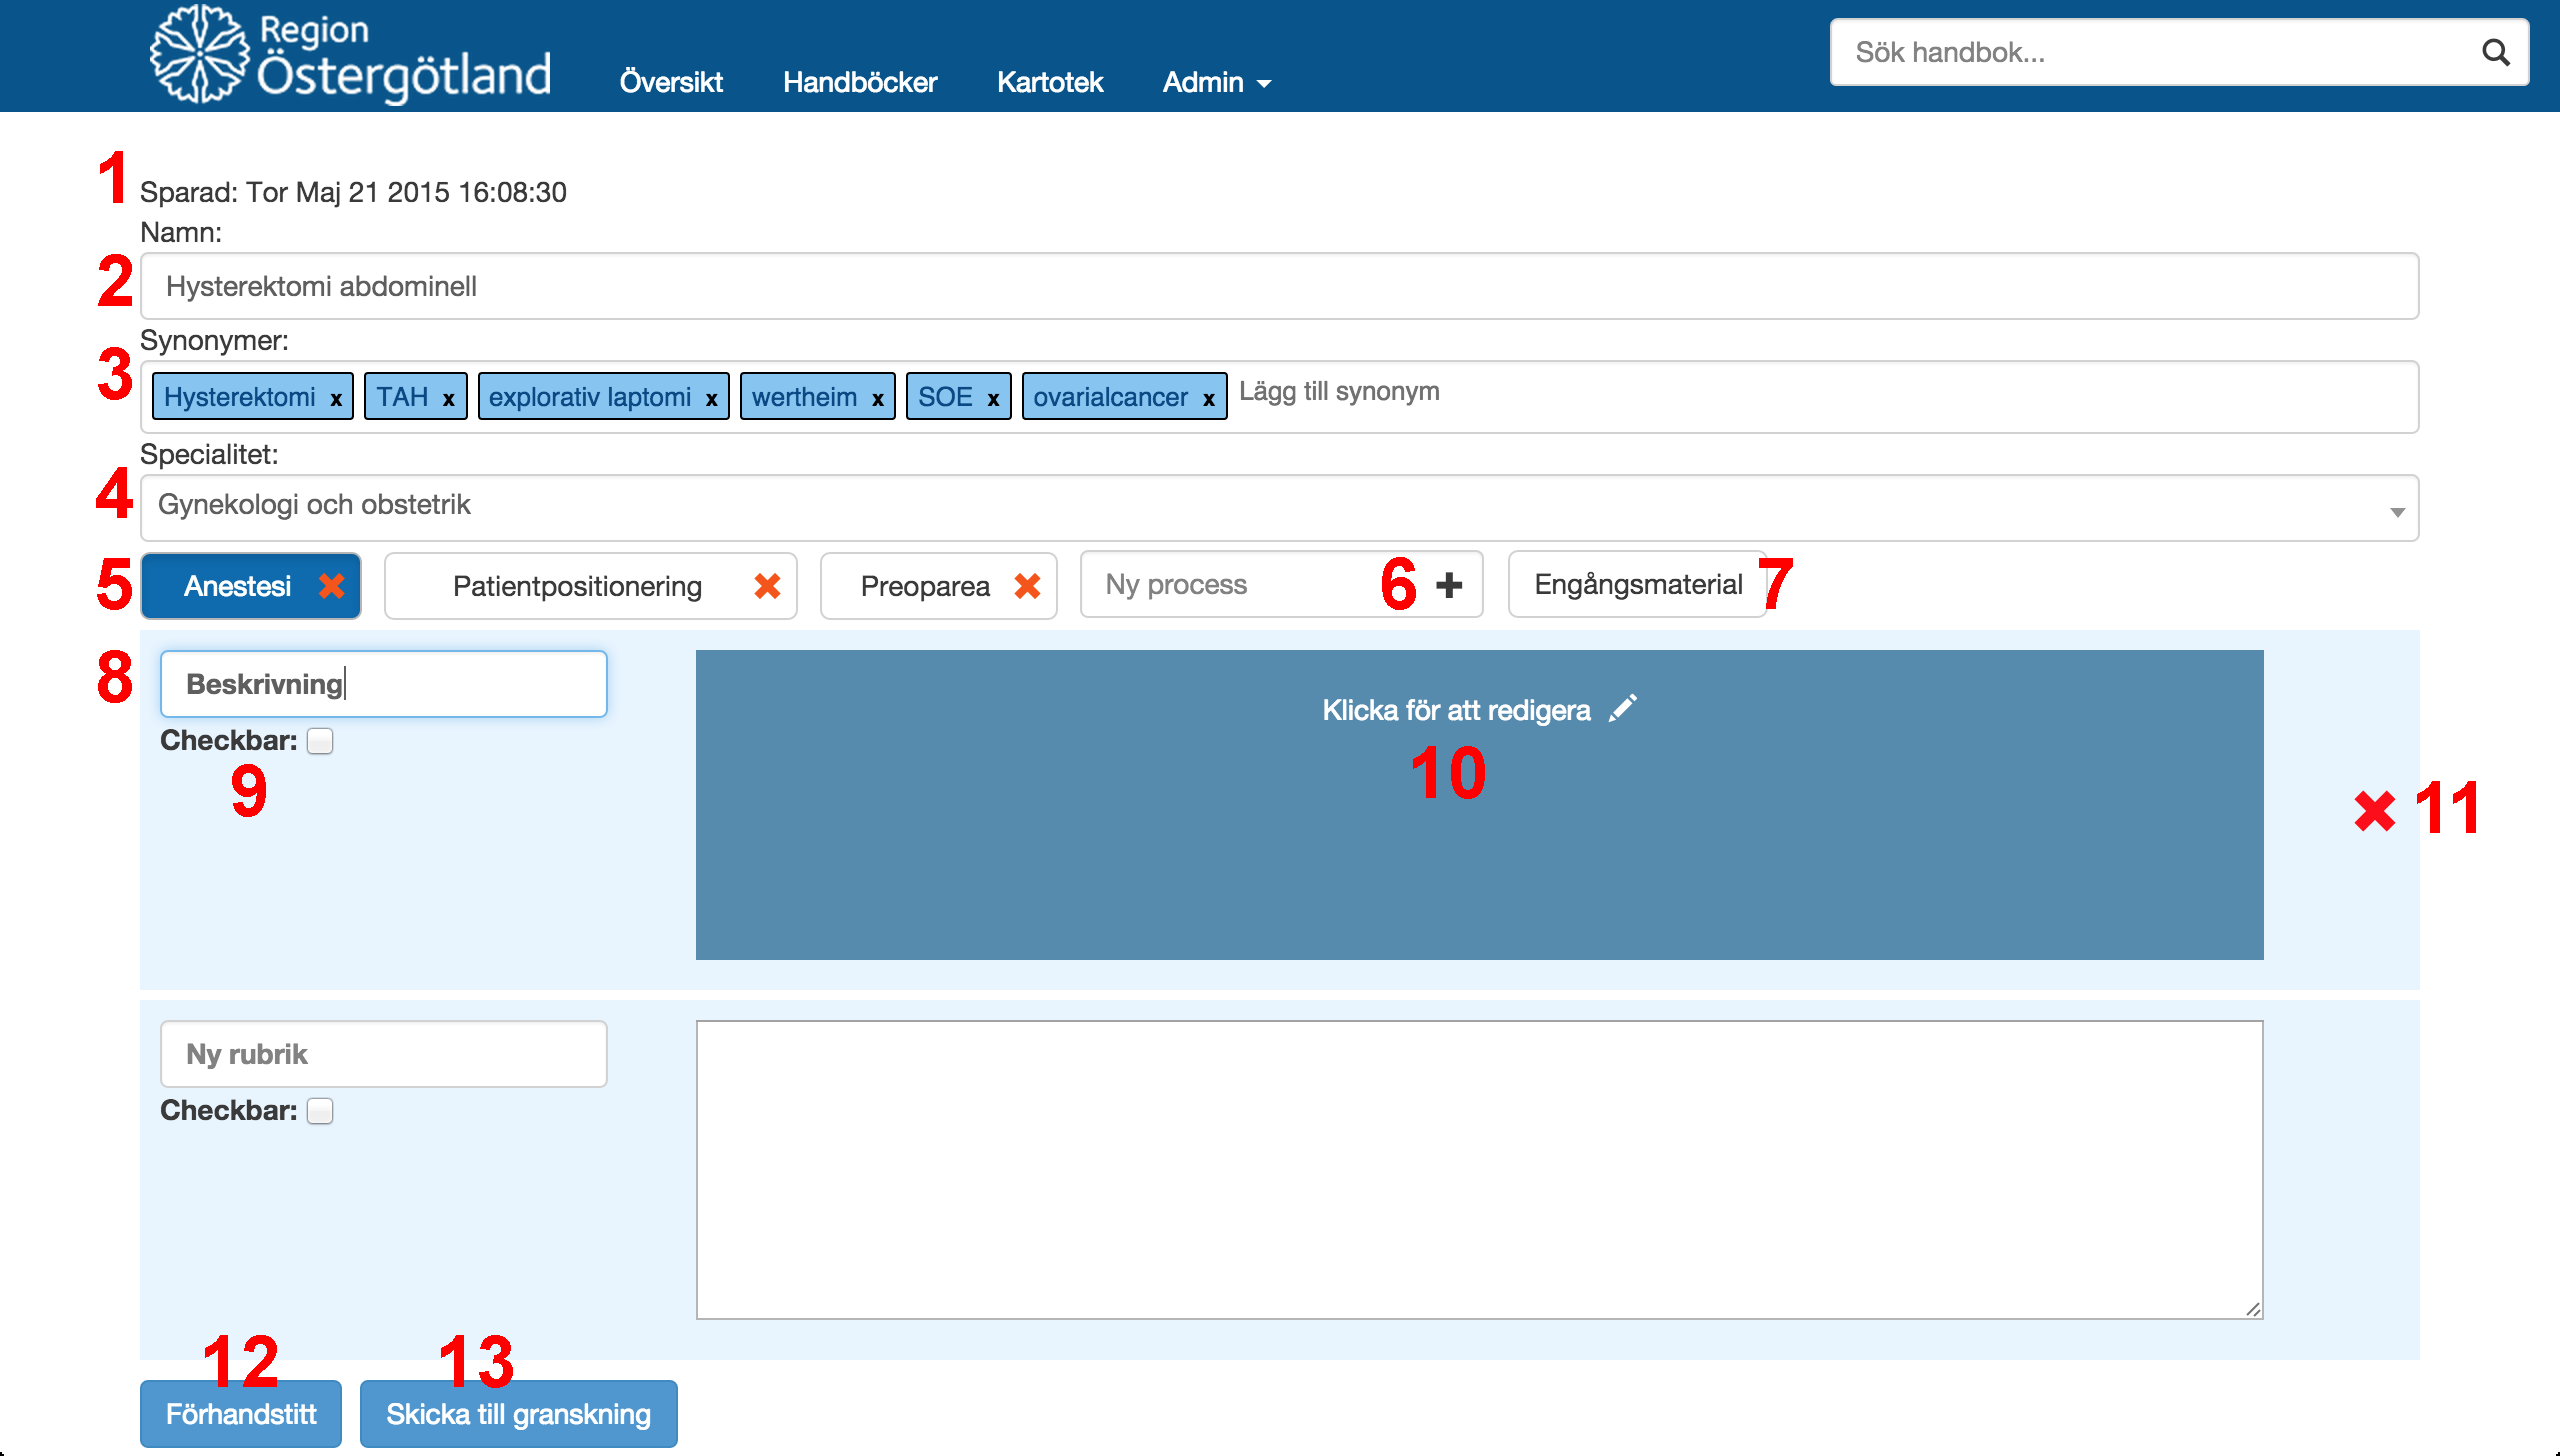
\includegraphics[scale=0.3]{redigeringsvy.png}
	\caption{Redigeringsvy}
	\label{fig:redigeringsvy}
	\end{center}
\end{figure}

\begin{enumerate}
\item Senaste redigeringsdatum.
\item Redigera handboksnamn.
\item Lägg till/ta bort synonymer.
\item Ändra specialitet.
\item Processteg. Klicka på ett processteg för att fylla i tillhörande rubriker. Krysset tar bort processteget. Kan sorteras genom klicka och dra.
\item Lägg till nytt processteg.
\item Flik för engångsmaterial. Denna flik finns alltid och kan inte tas bort. Se mer under rubriken ''Engångsmaterial''.
\item Underrubriksnamn. När man börjar fylla i ett namn skapas en ny rubrik underst. Underrubrikerna kan sorteras genom att klicka och dra.
\item Kryssa i om rubriken ska vara checkbar.
\item Klicka här för att få upp redigering av rubriksinnehåll. Se mer under rubriken ''Rubriksinnehåll''.
\item Krysset tar bort underrubriken.
\item Gå till förhandstitt.
\item Skickar handboken till granskning.
\end{enumerate}

\subsection{Engångsmaterial}
Figur \ref{fig:engangsmaterial} visar fliken engångsmaterial. Här skapar man plocklistan.

\begin{figure}[H]
	\begin{center}
	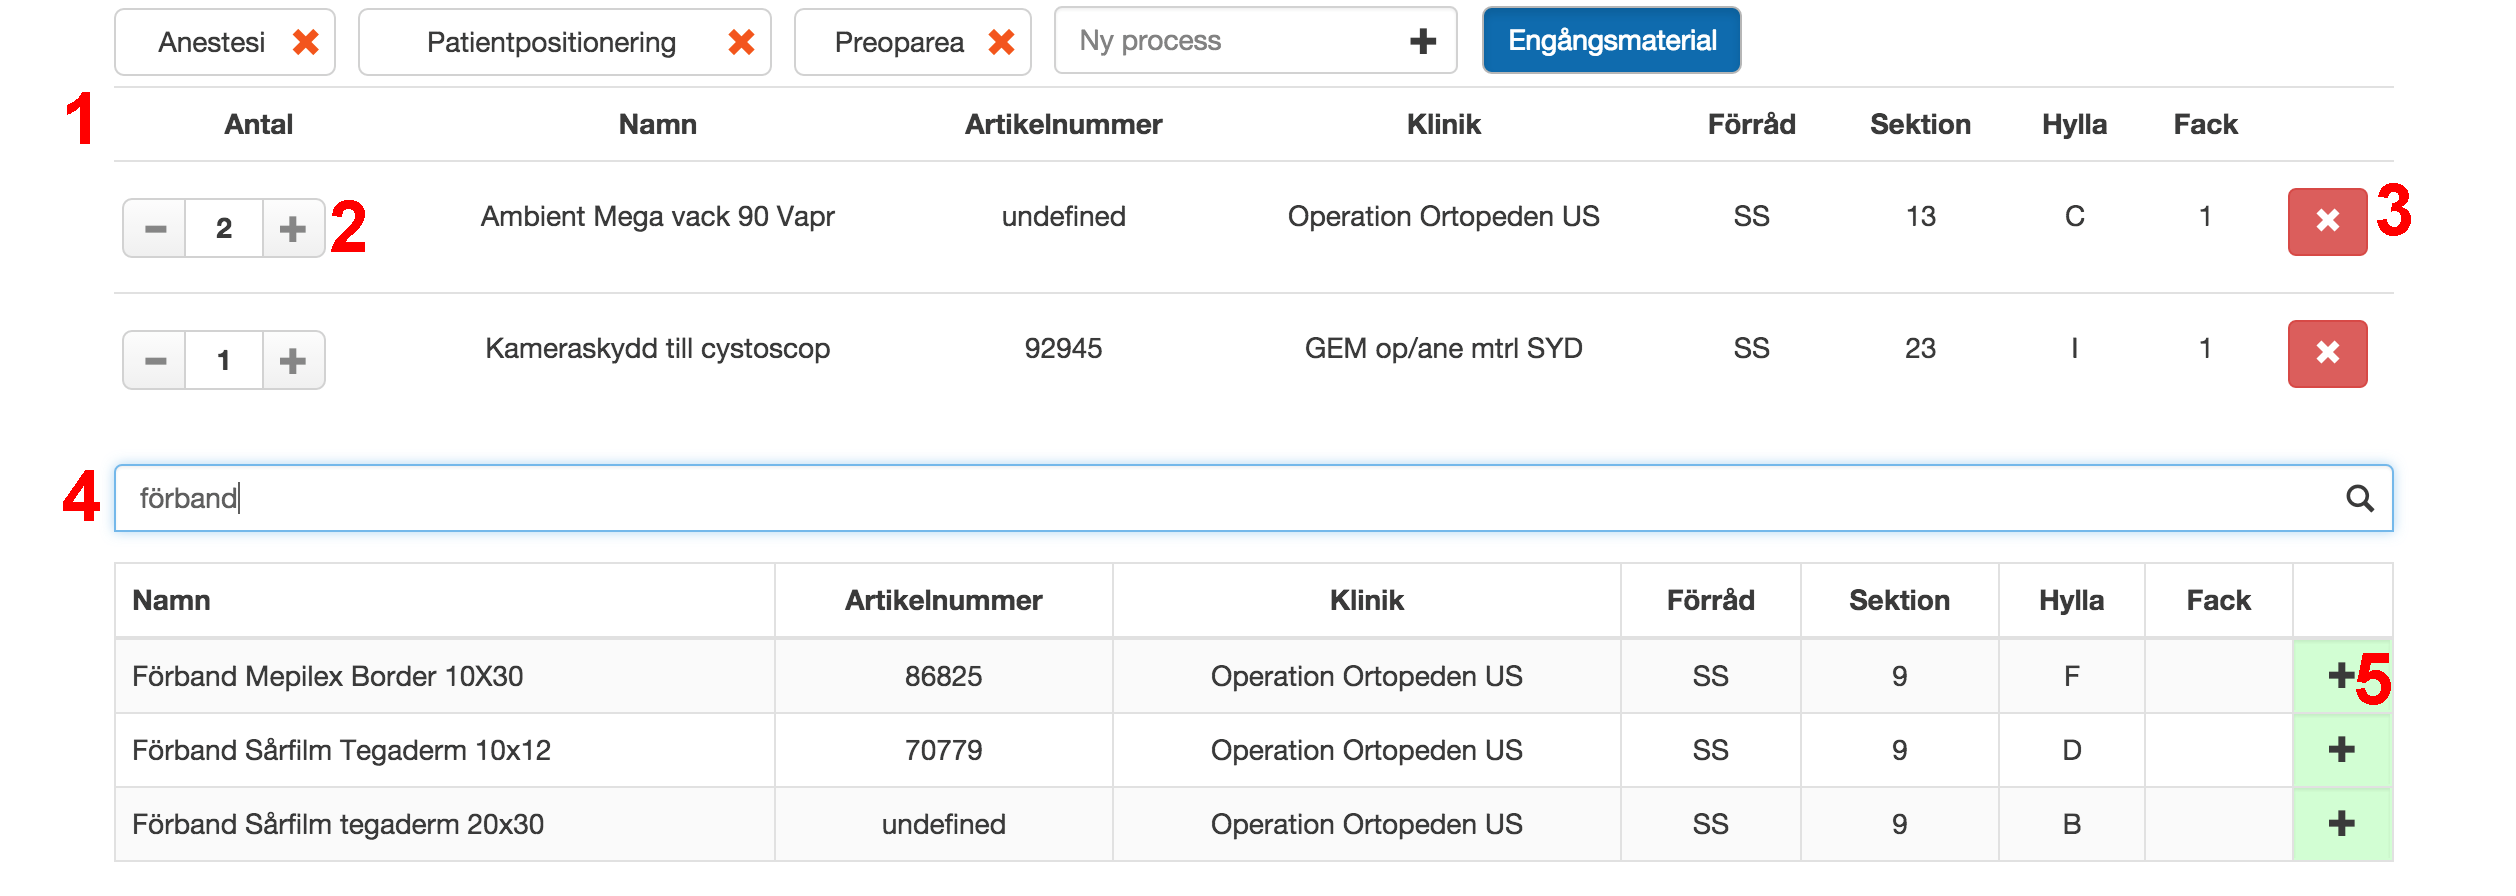
\includegraphics[scale=0.3]{engangsmaterial.png}
	\caption{Engangsmaterial}
	\label{fig:engangsmaterial}
	\end{center}
\end{figure}

\begin{enumerate}
\item Tabell med engångsmaterial.
\item Redigera antal.
\item Ta bort artikel.
\item Sök på artikel i kartoteket.
\item Lägg till artikel. Kan också klicka vartsomhelst på raden.

\end{enumerate}

\subsection{Rubriksinnehåll}


I figur \ref{fig:rubriksinnehall} visas hur redigering av rubriksinnehåll ser ut. Det fungerar i princip på samma sätt som en vanlig ordbehandlare. Man kan formatera innehållet med punktlistor, tabeller etc. Man kan också lägga in bilder och video, antingen direkt från hårddisk eller från länk på internet.

\begin{figure}[H]
	\begin{center}
	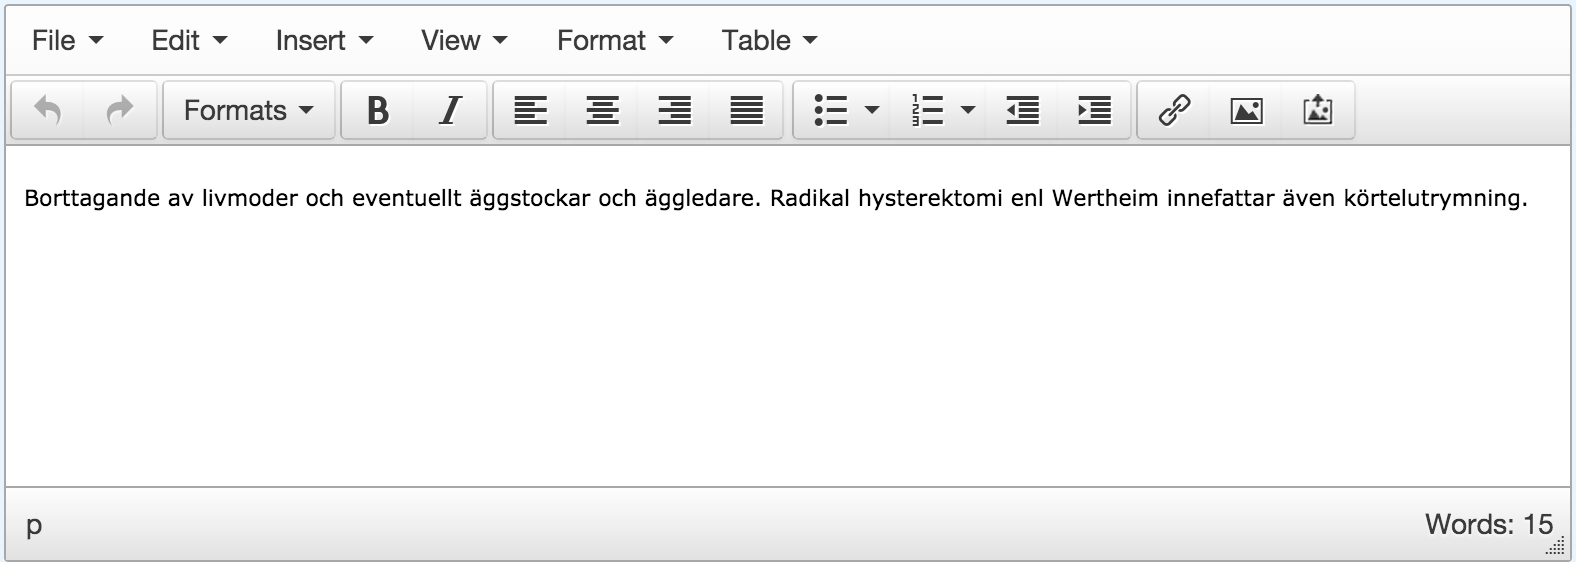
\includegraphics[scale=0.5]{rubriksinnehall.png}
	\caption{Rubriksinnehåll}
	\label{fig:rubriksinnehall}
	\end{center}
\end{figure}

För att lägga in bilder eller video kan man gå till menyn insert ( se figur \ref{fig:insert} ).

\begin{figure}[H]
	\begin{center}
	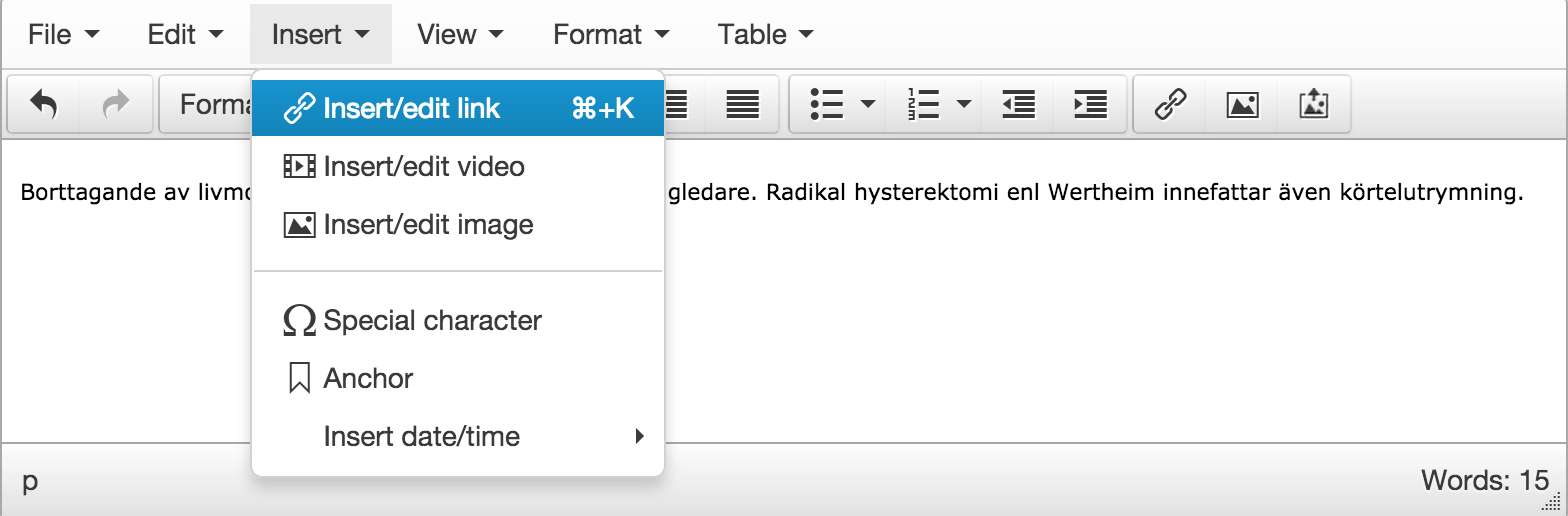
\includegraphics[scale=0.5]{insert.png}
	\caption{Insert}
	\label{fig:insert}
	\end{center}
\end{figure}

I figur \ref{fig:general} visas hur man kan lägga in video från länk på internet.

\begin{figure}[H]
	\begin{center}
	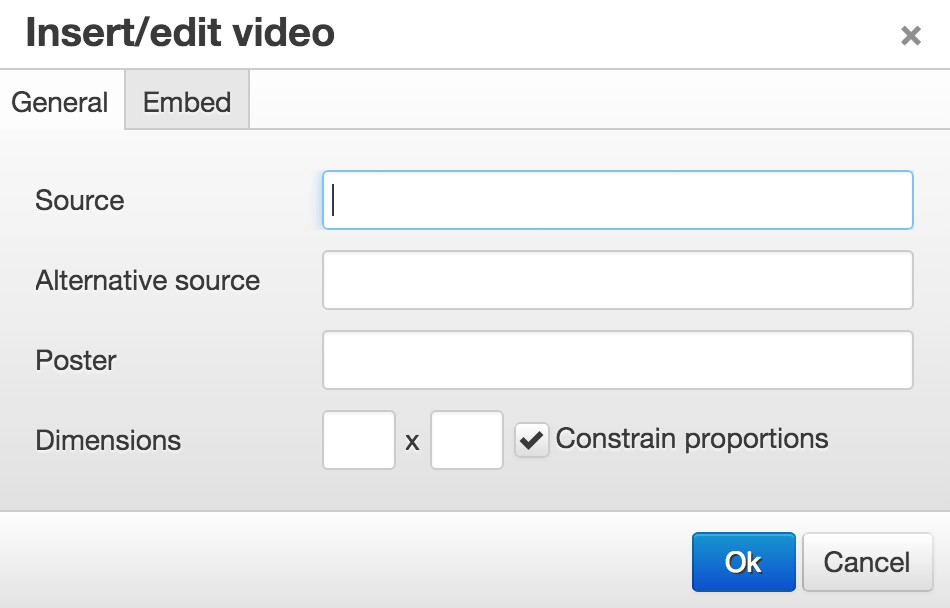
\includegraphics[scale=0.5]{general.png}
	\caption{Lägg in video från source}
	\label{fig:general}
	\end{center}
\end{figure}

I figur \ref{fig:embed} visas hur man kan lägga in video genom att bädda in kod.

\begin{figure}[H]
	\begin{center}
	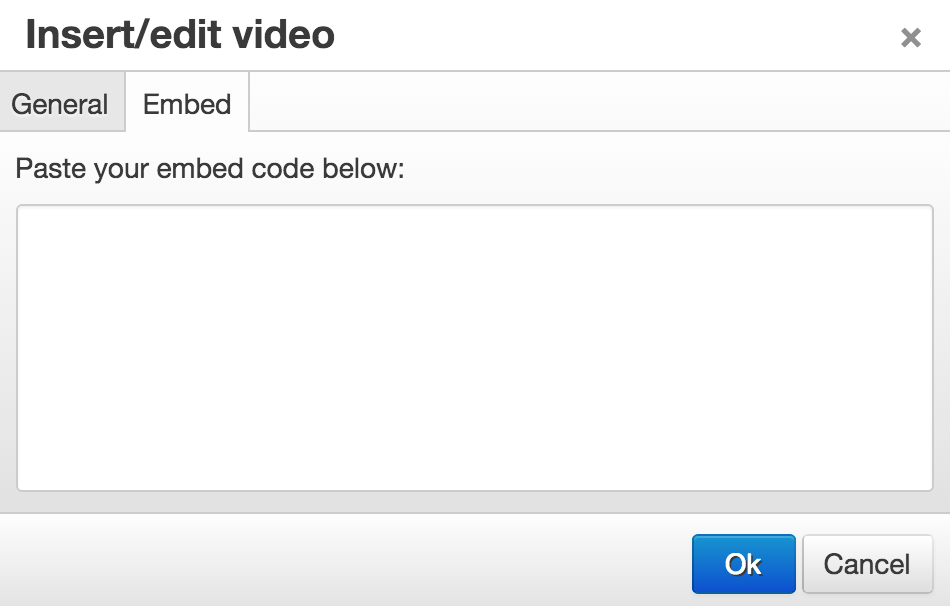
\includegraphics[scale=0.5]{embed.png}
	\caption{Lägg in video med inbäddad kod}
	\label{fig:embed}
	\end{center}
\end{figure}

\section{Kartoteket}
I figur \ref{fig:kartoteket} visas kartoteket.

  \begin{figure}[H]
	\begin{center}
	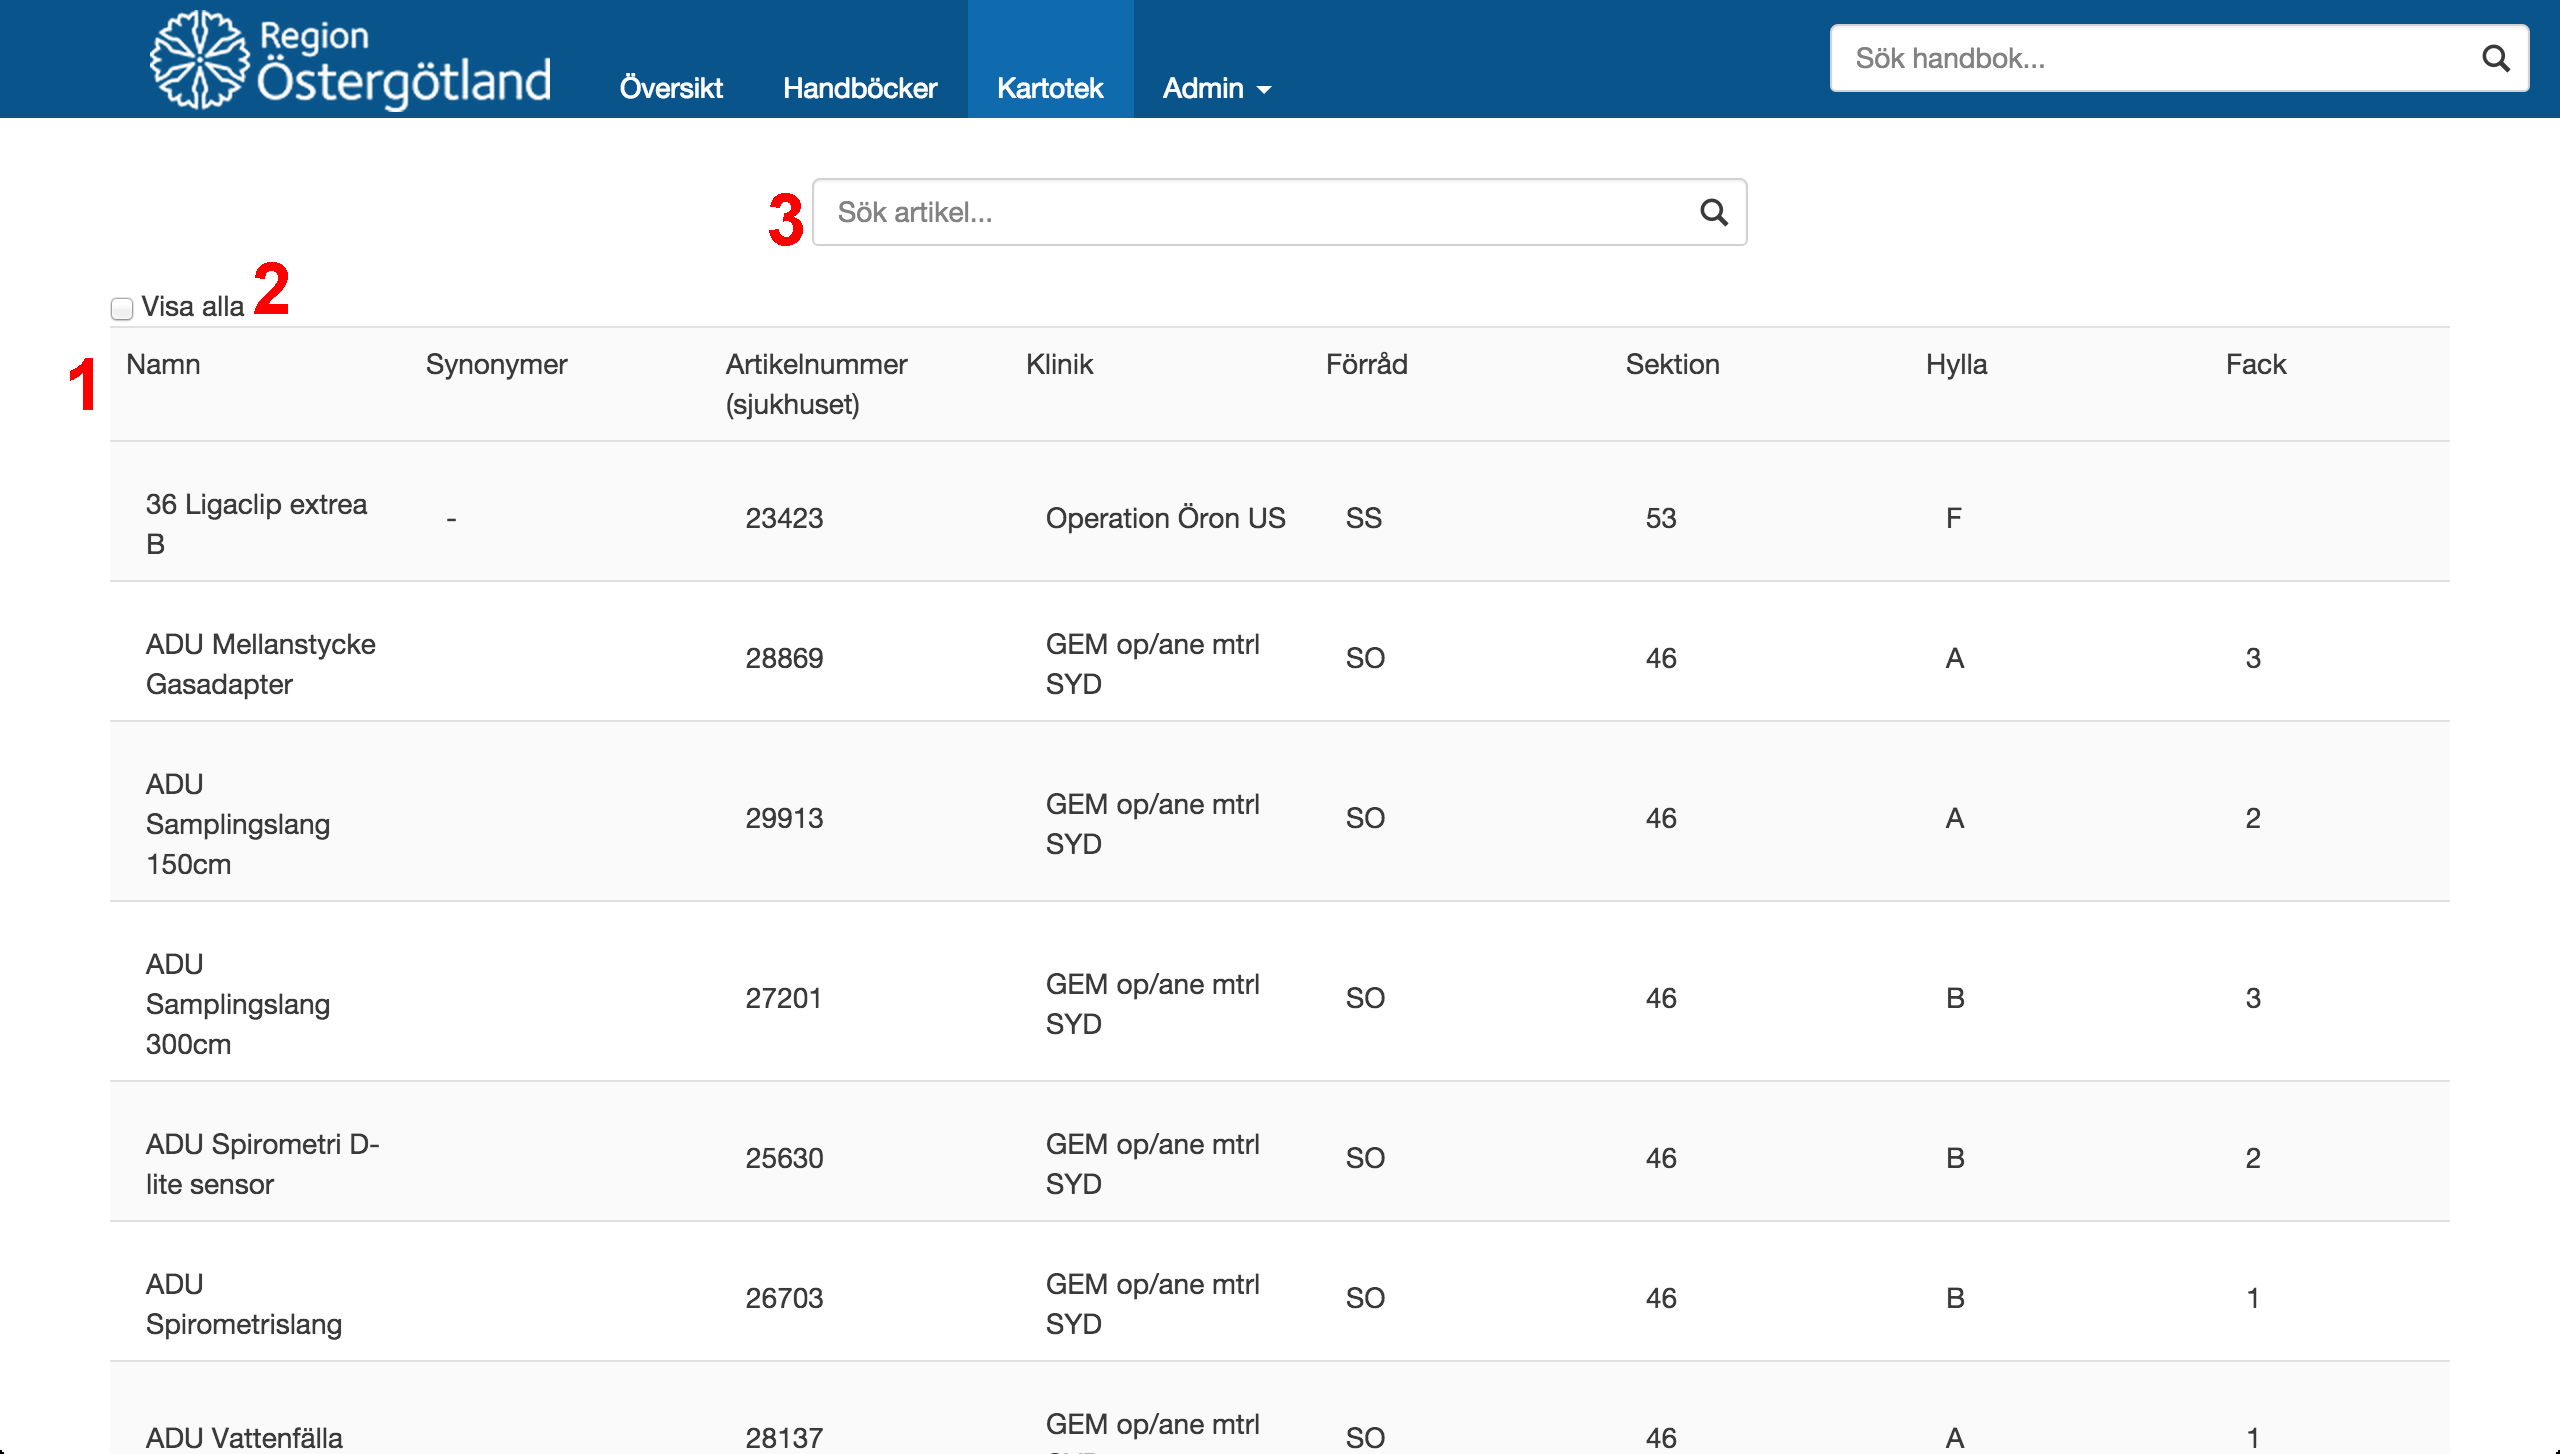
\includegraphics[scale=0.3]{kartoteket.png}
	\caption{Kartoteket}
	\label{fig:kartoteket}
	\end{center}
\end{figure}

\begin{enumerate}
\item En tabell innehållande alla artiklar med tillhörande information.
\item Kryssa i ''Visa alla'' för att visa extra information om artiklarna t.ex. pris. Med denna ikryssad kan man också lägga till nya artiklar.
\item Här kan man söka på artiklar.
\end{enumerate}
\subsection{Redigering}
Figur \ref{fig:kartotekredigering1} och figur \ref{fig:kartotekredigering2} visar hur man kan lägga till och redigera en artikel. I figur \ref{fig:kartotekredigering2} har vi scrollat till höger.

 \begin{figure}[H]
	\begin{center}
	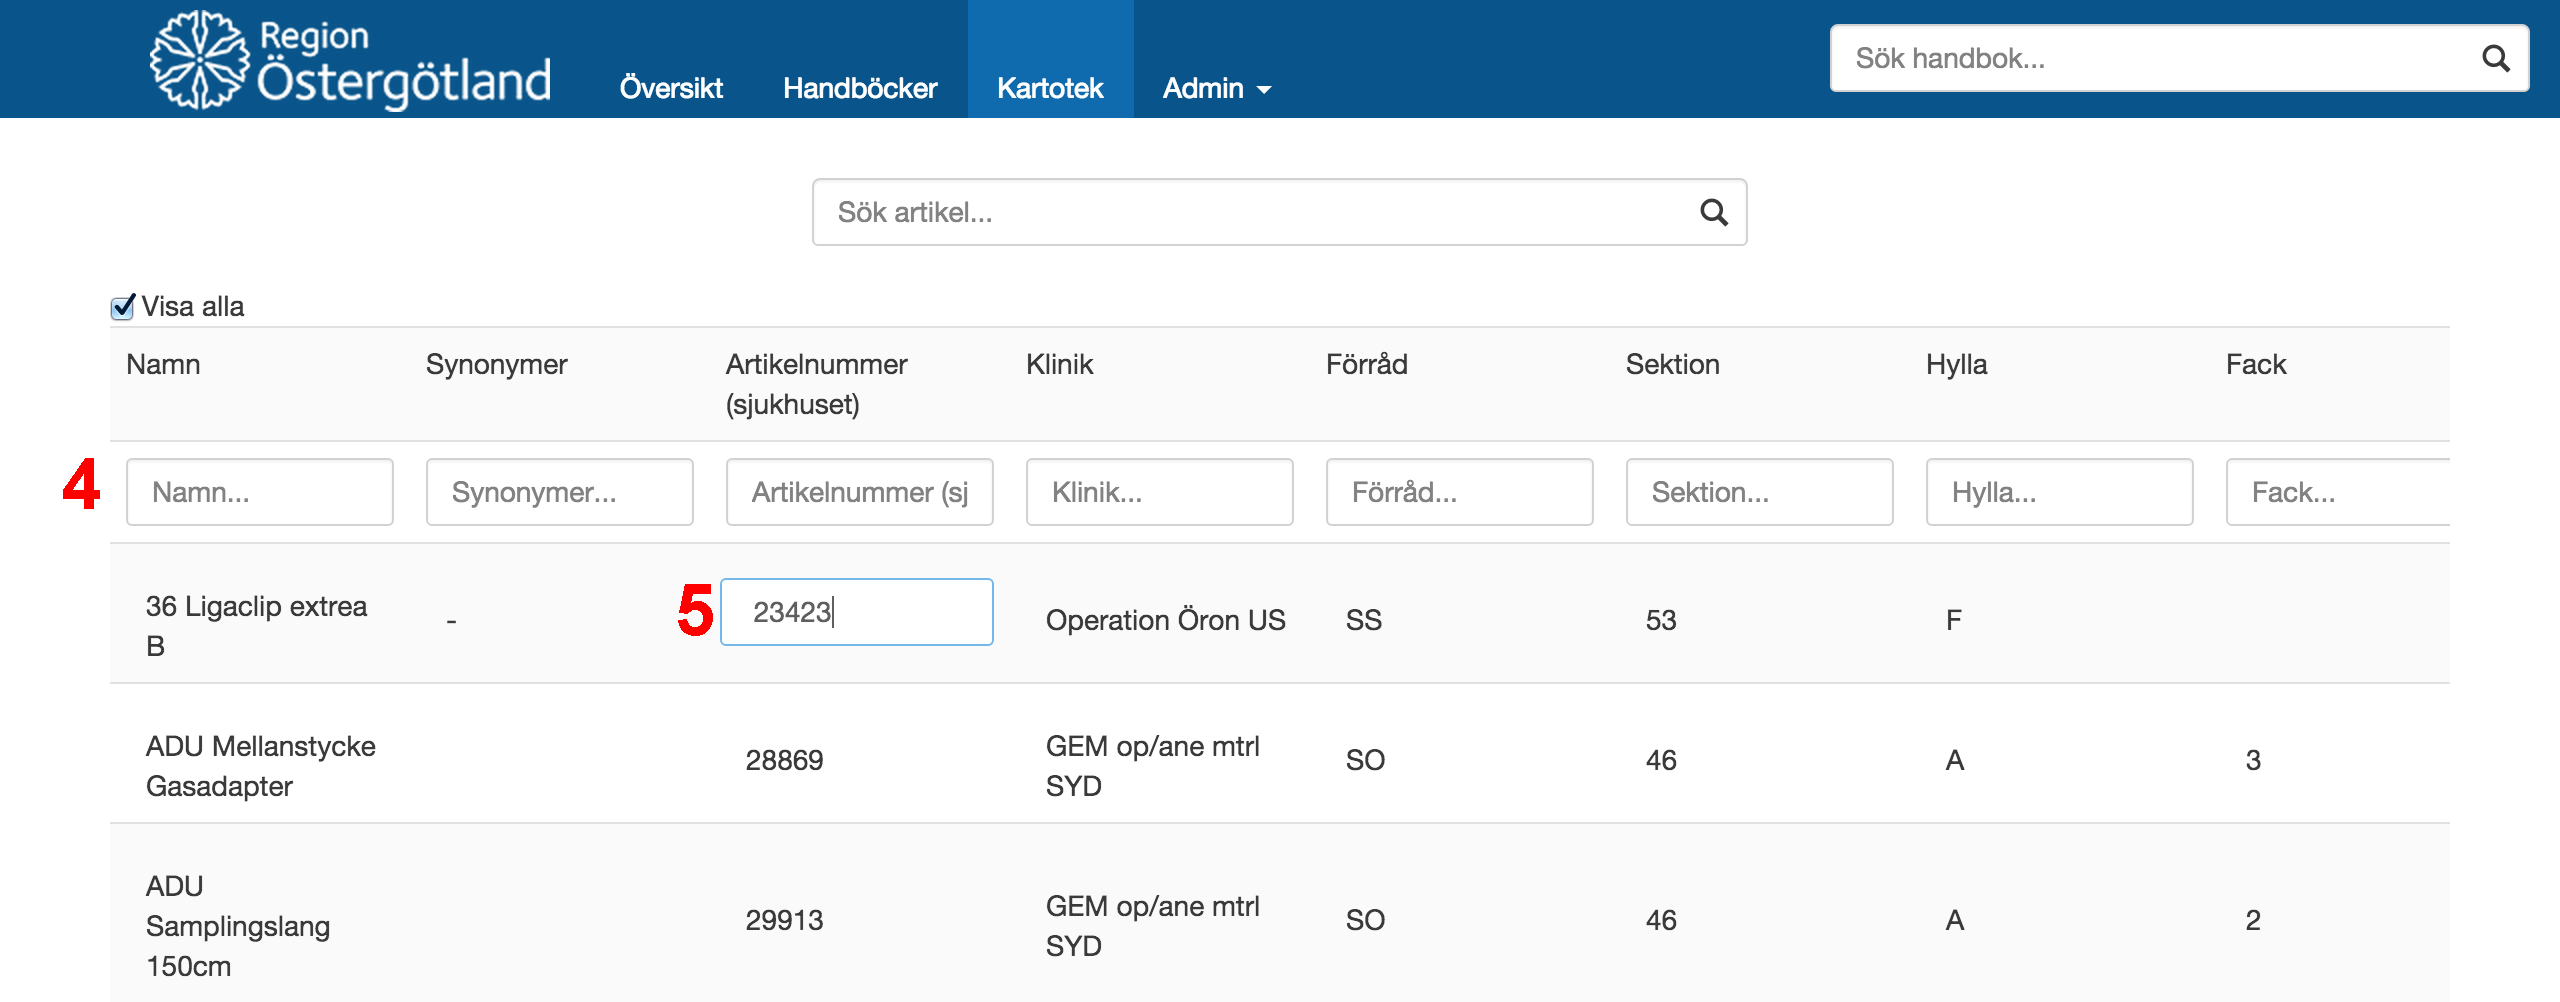
\includegraphics[scale=0.3]{kartotekredigering1.png}
	\caption{Redigering i Kartoteket}
	\label{fig:kartotekredigering1}
	\end{center}
\end{figure}

 \begin{figure}[H]
	\begin{center}
	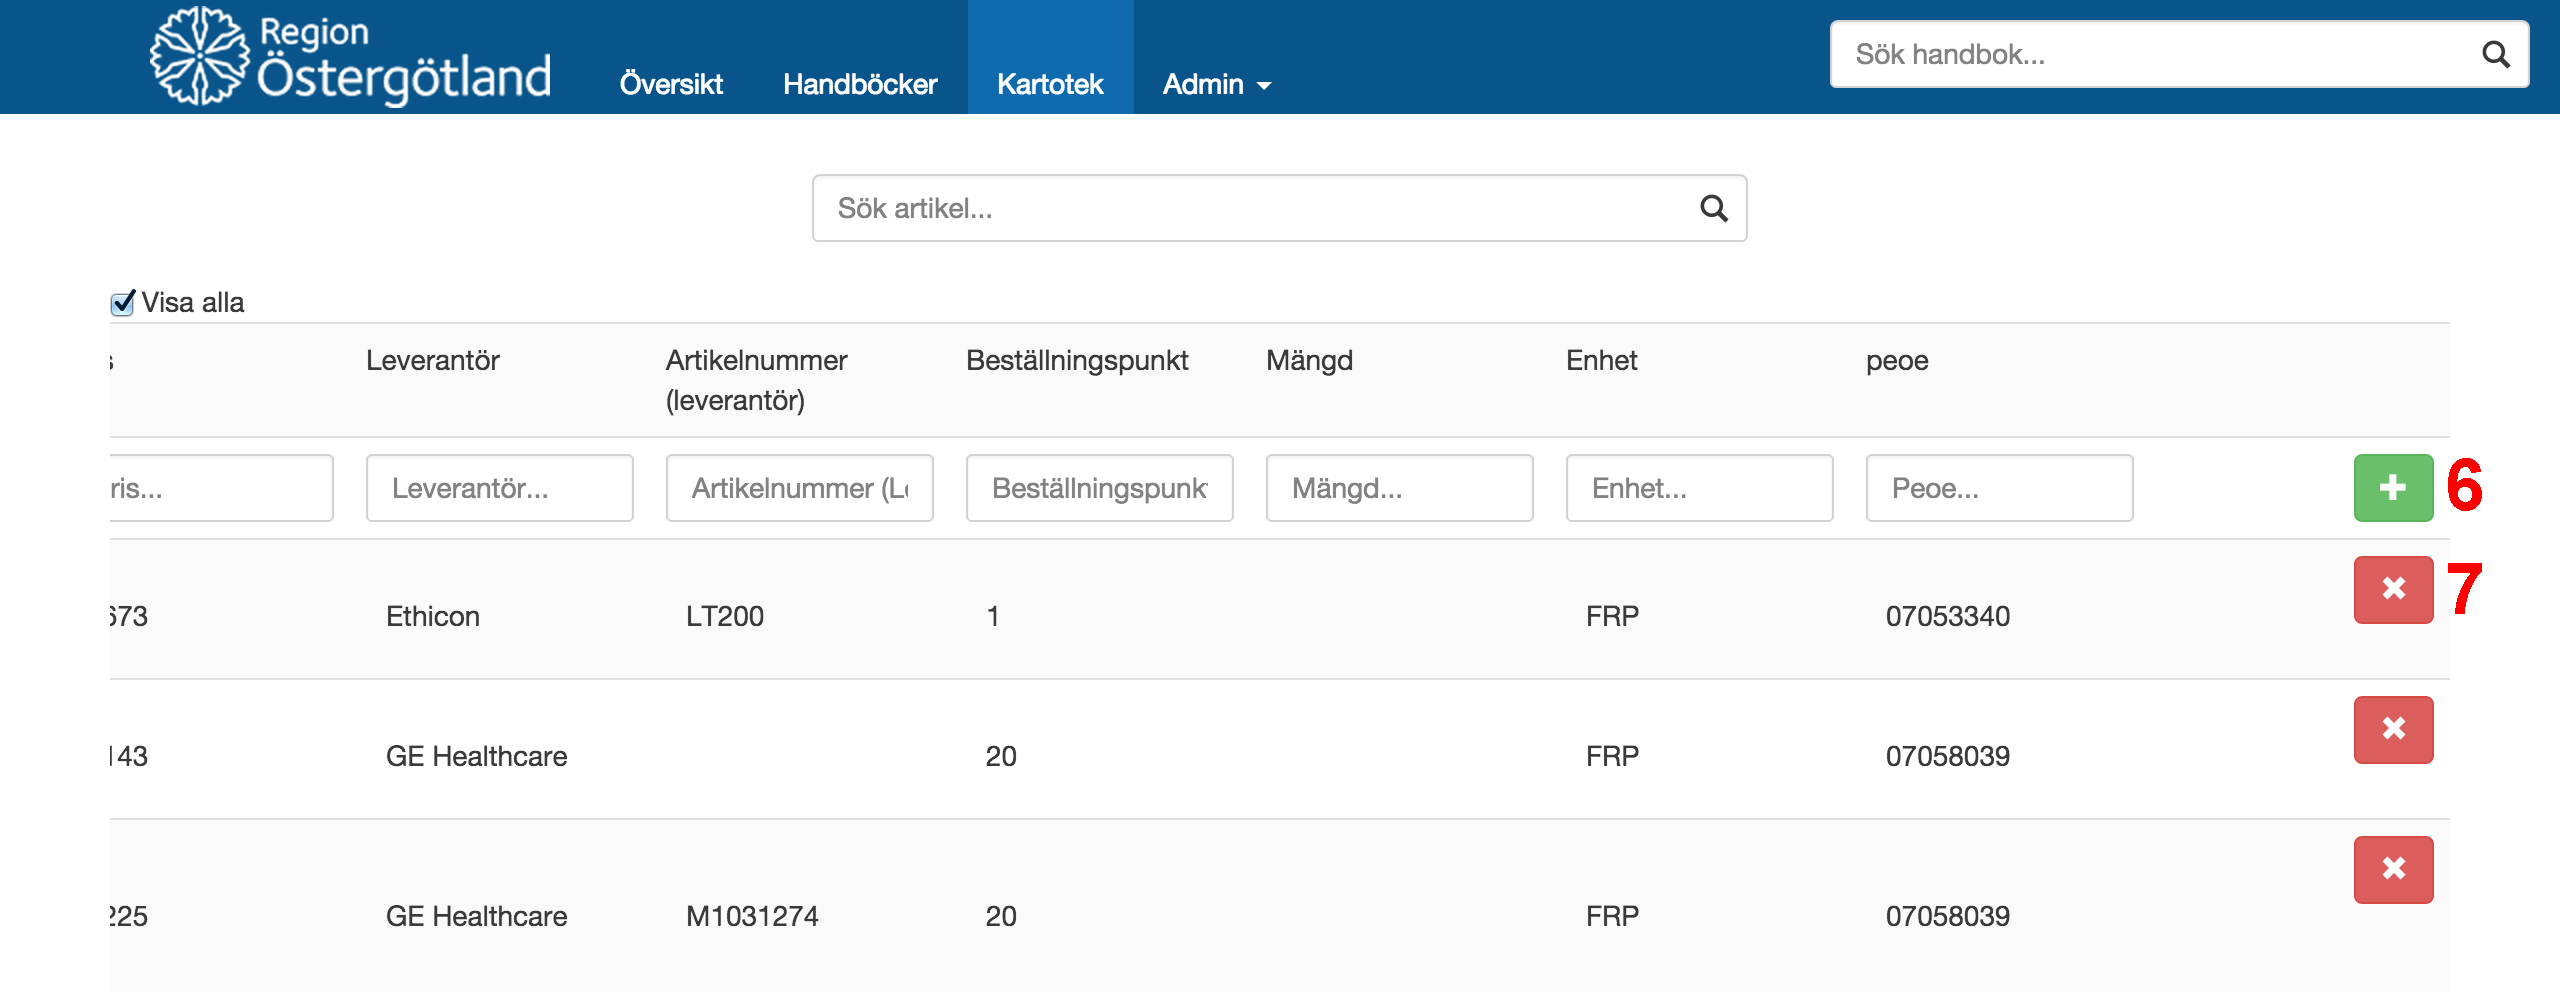
\includegraphics[scale=0.3]{kartotekredigering2.png}
	\caption{Redigering i Kartoteket, scrollat till höger}
	\label{fig:kartotekredigering2}
	\end{center}
\end{figure}

\begin{enumerate}
  \setcounter{enumi}{3}
  \item Fält för ny artikel. 
  \item Klicka på ett fält för att redigera det.
  \item Lägg till ny artikel. Observera att pris måste vara angivet.
  \item Ta bort artikel.
\end{enumerate}

\section{Översiktsvyn}

I figur \ref{fig:overview} visas översiktsvyn med pågående operationsförberedelser.

 \begin{figure}[H]
	\begin{center}
	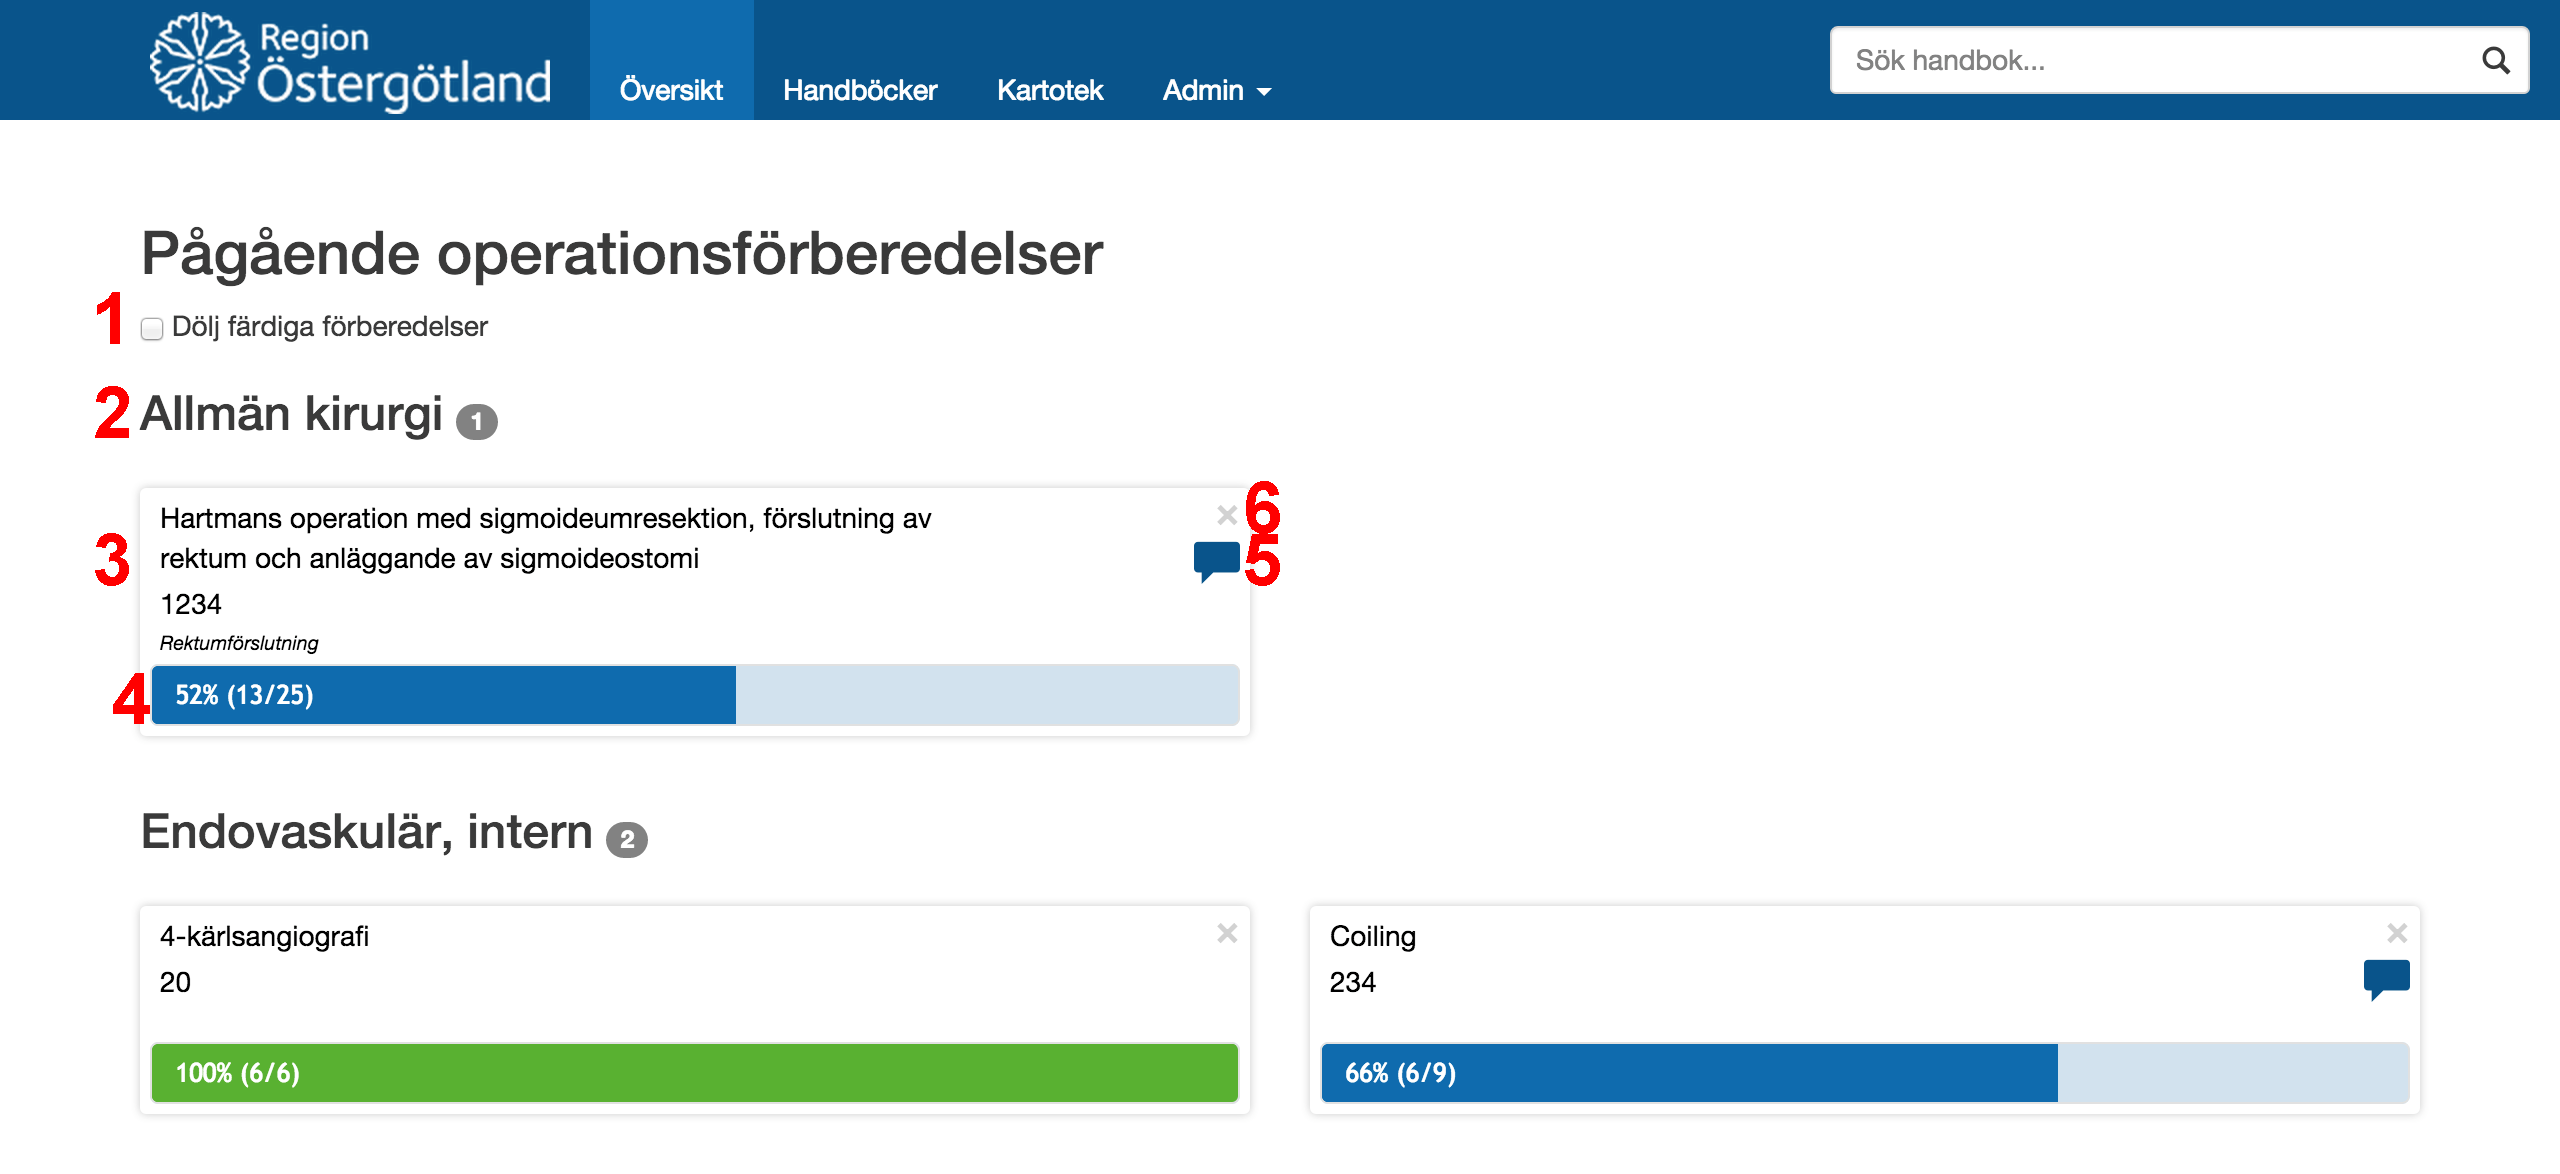
\includegraphics[scale=0.3]{overview.png}
	\caption{Översiktsvyn}
	\label{fig:overview}
	\end{center}
\end{figure}

\begin{enumerate}
\item Kryssa i för att dölja färdiga operationsförberedelser.
\item Operationsförberedelserna sorteras under dess specialitéer. Numret till höger visar hur många operationsförberedelser som finns för denna specialitet.
\item En operationsförberedelse. Texten är handboksnamn, linda-id och synonymer. 
\item Denna statusbar visar summan av plockat engångsmaterial och förberedda förberedelser.
\item Klicka på denna ikon för att visa kommentarer för artiklar.
\item Krysset tar bort operationsförberedelsen.

\end{enumerate}

\section{Operationsförberedelse}
En operationsförberedelse visas i figur \ref{fig:opforberedelse}. Dessa nås genom översiktsvyn. 

\begin{figure}[H]
	\begin{center}
	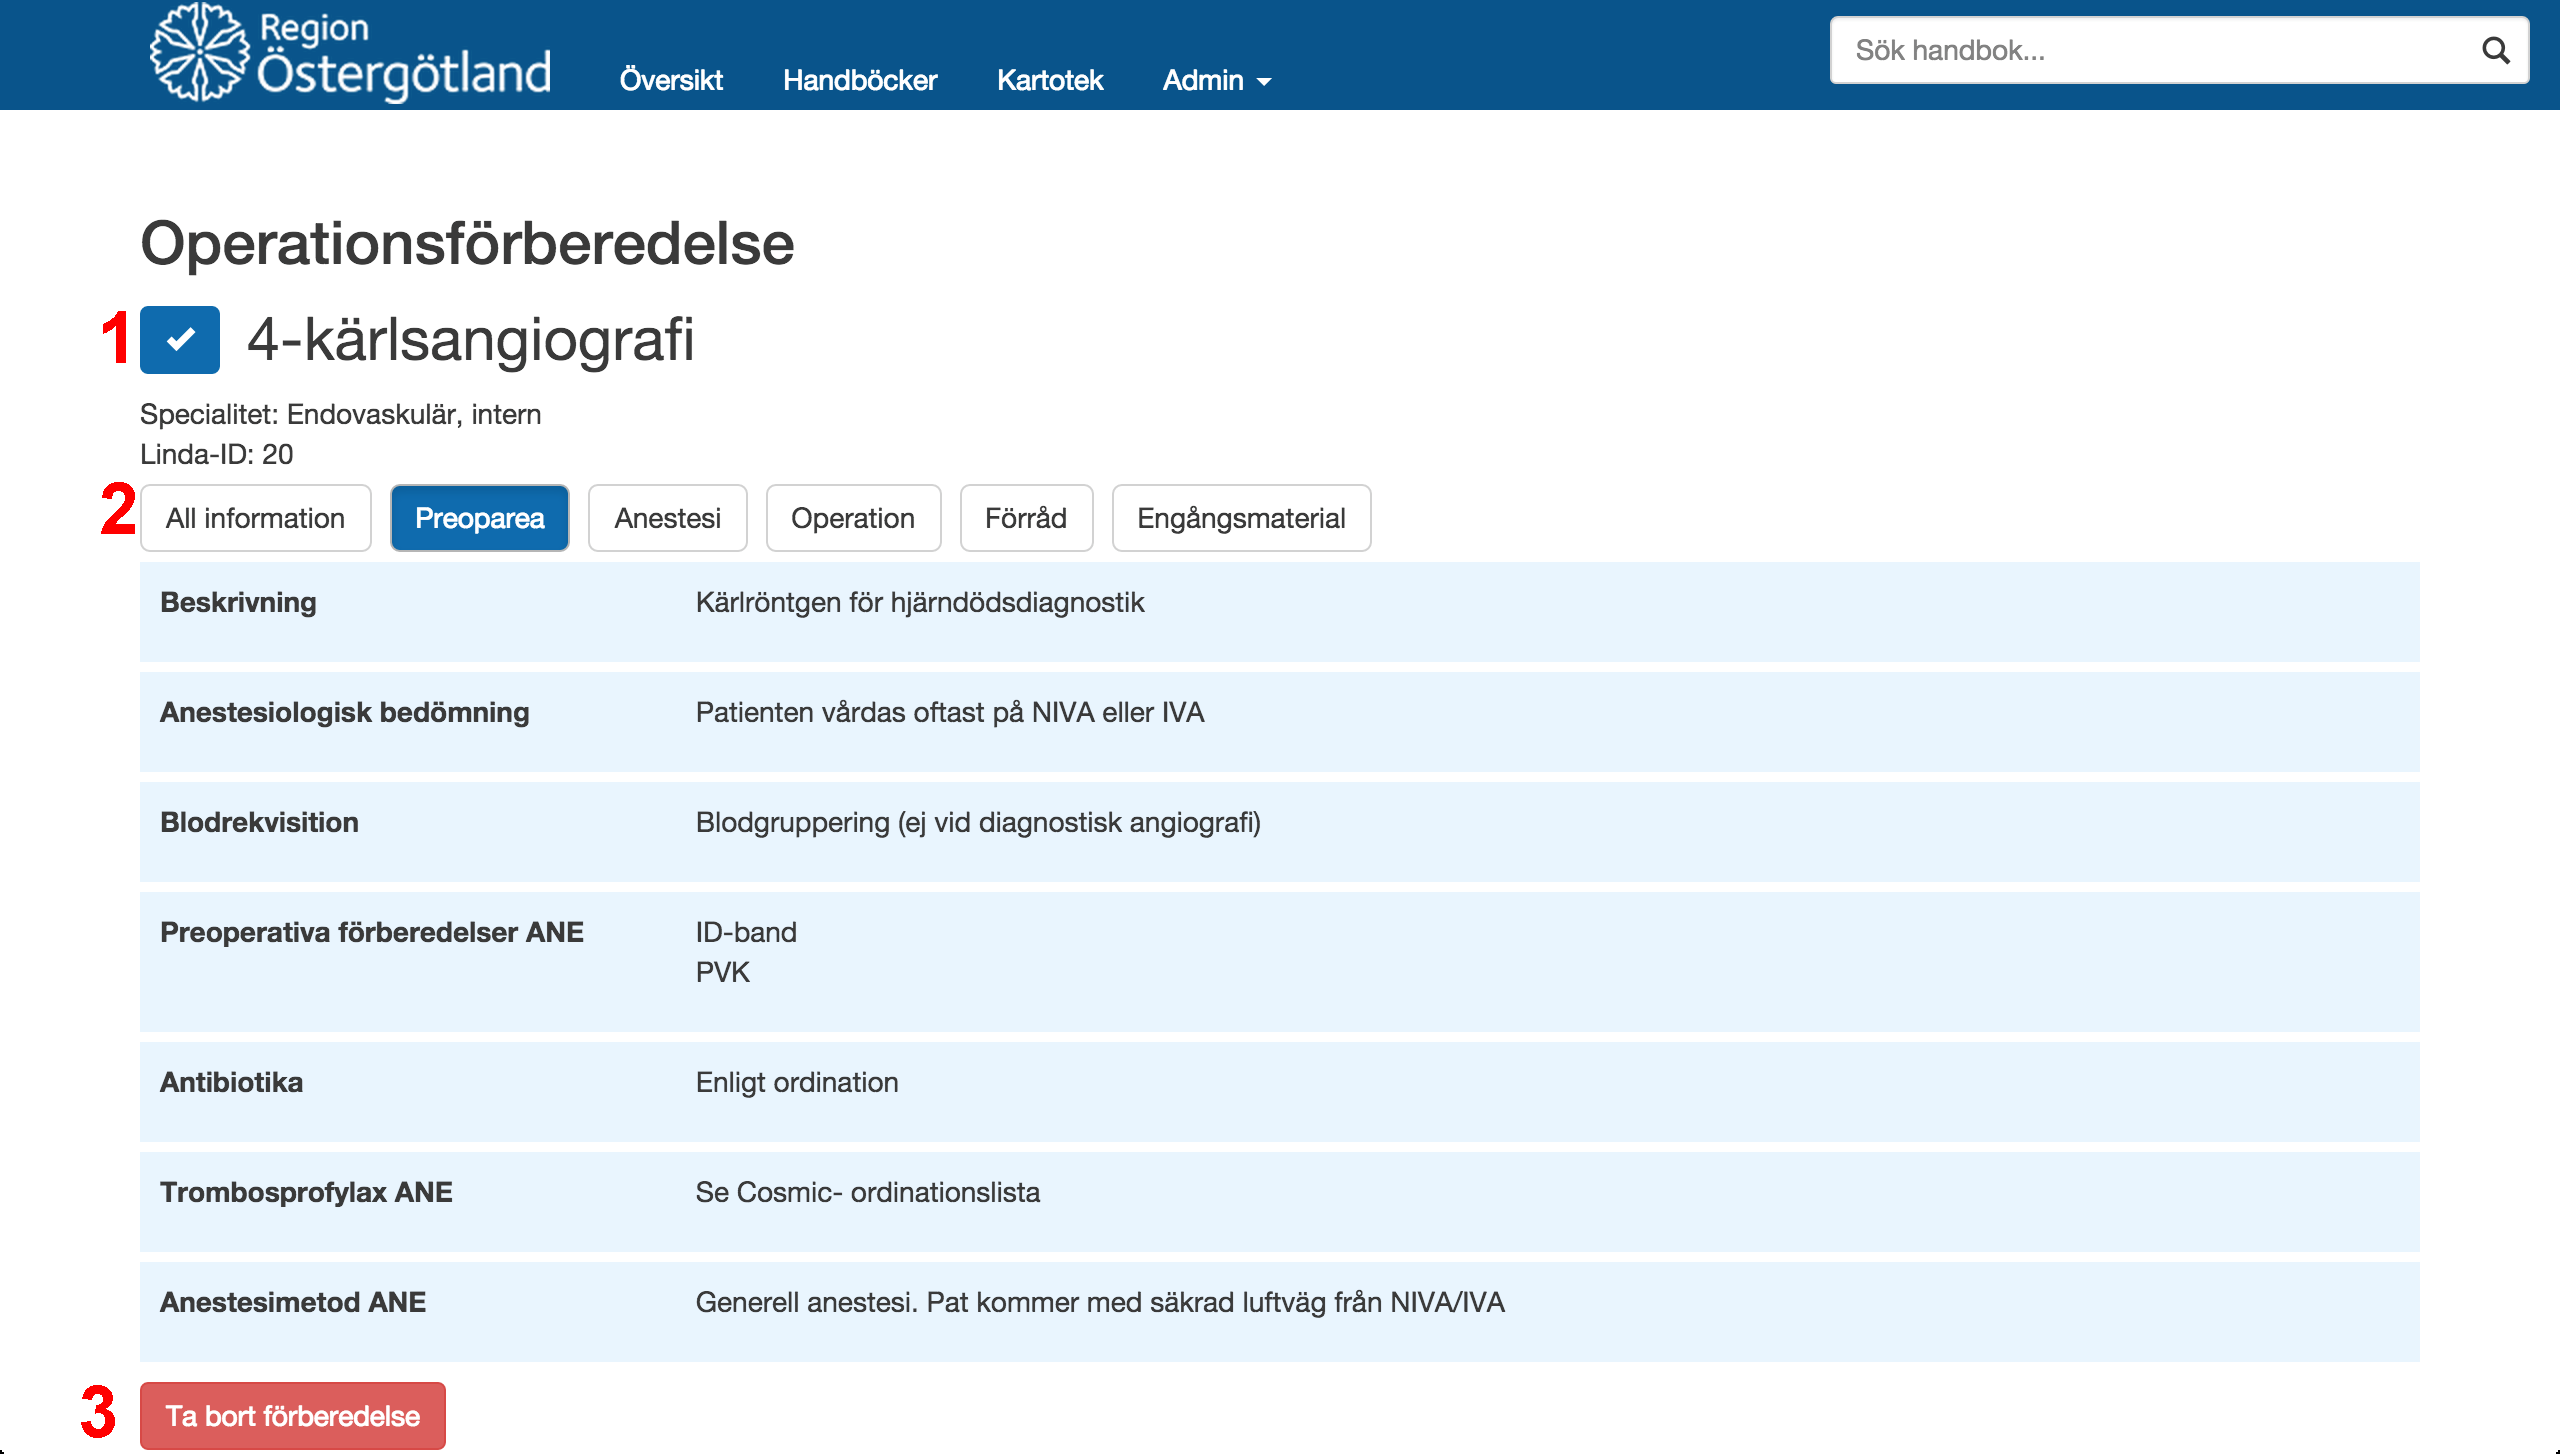
\includegraphics[scale=0.3]{opforberedelse.png}
	\caption{Operationsförberedelse}
	\label{fig:opforberedelse}
	\end{center}
\end{figure}

\begin{enumerate}
\item Denna knapp kan klickas för att visa att operationsförberedelsen är klar även om alla artiklar inte checkats. Statusbaren på översiktsvyn blir grön.
\item Flikar med tillhörande underrubriker för de olika processtegen.
\item Tar bort operationsförberedelsen.
\end{enumerate}

\subsection{Engångsmaterial}
I figur \ref{fig:opforberedelse_engangsmaterial} visas fliken engånsmaterial där plocklistan finns.

\begin{figure}[H]
	\begin{center}
	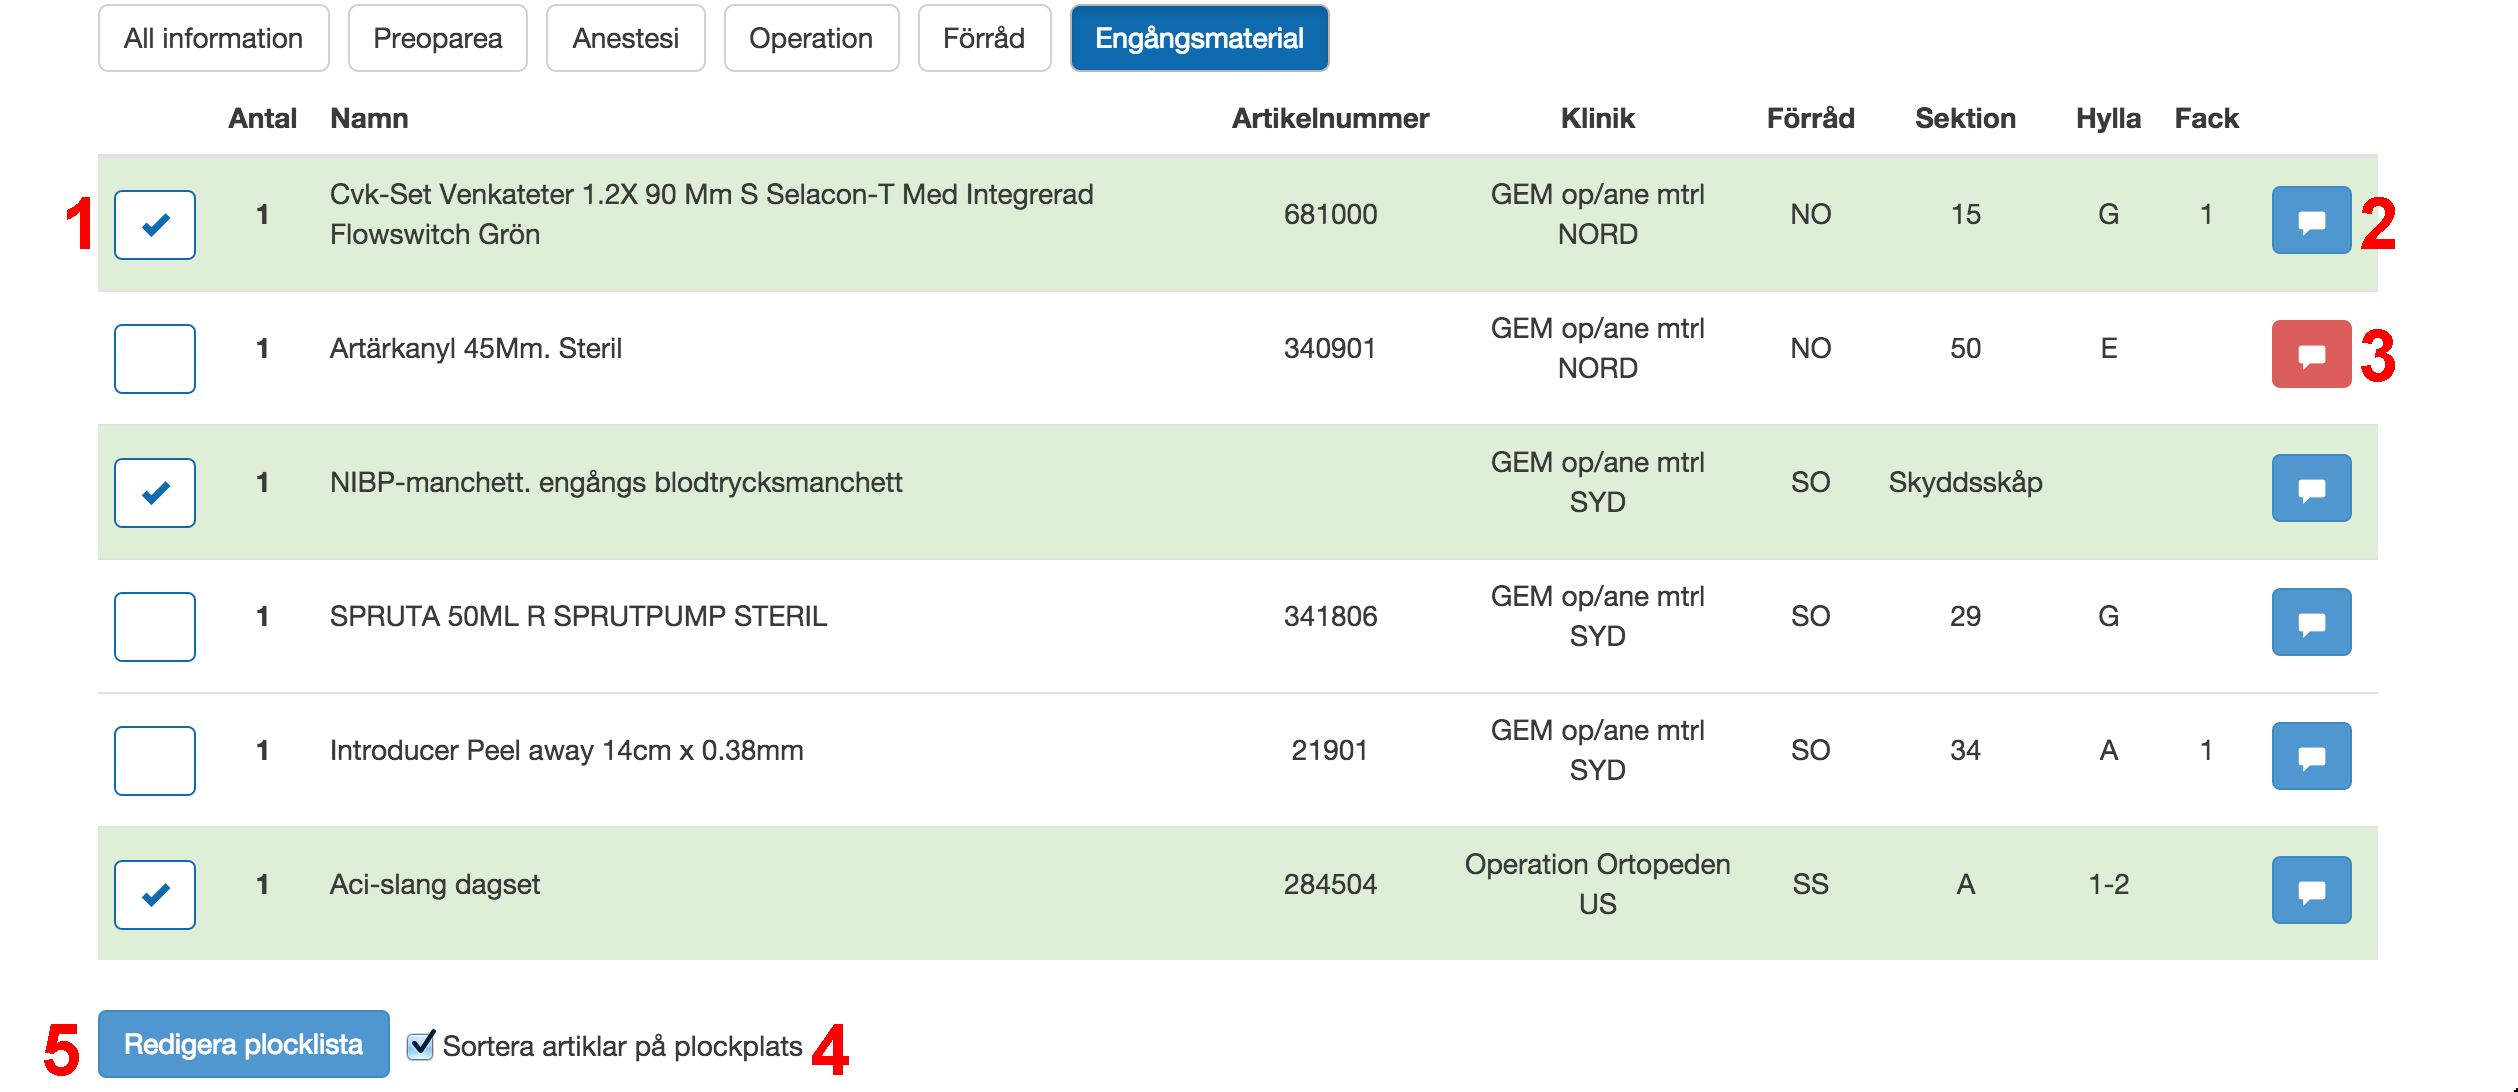
\includegraphics[scale=0.3]{opforberedelse_engangsmaterial.png}
	\caption{Plocklista}
	\label{fig:opforberedelse_engangsmaterial}
	\end{center}
\end{figure}

\begin{enumerate}
\item Klicka för att checka av plockad artikel.
\item Klicka för att lägga till kommentar på artikeln.
\item Röd ikon visar att det finns en kommentar.
\item Kryssa i för att sortera artiklarna på plockplats. Standard är sortering på namn.
\item Klicka för att kunna redigera antal artiklar eller lägga till/ta bort en artikel.
\end{enumerate}

\section{Hitta handböcker}
I figur \ref{fig:handbok} visas hur alla handböcker listas.

\begin{figure}[H]
	\begin{center}
	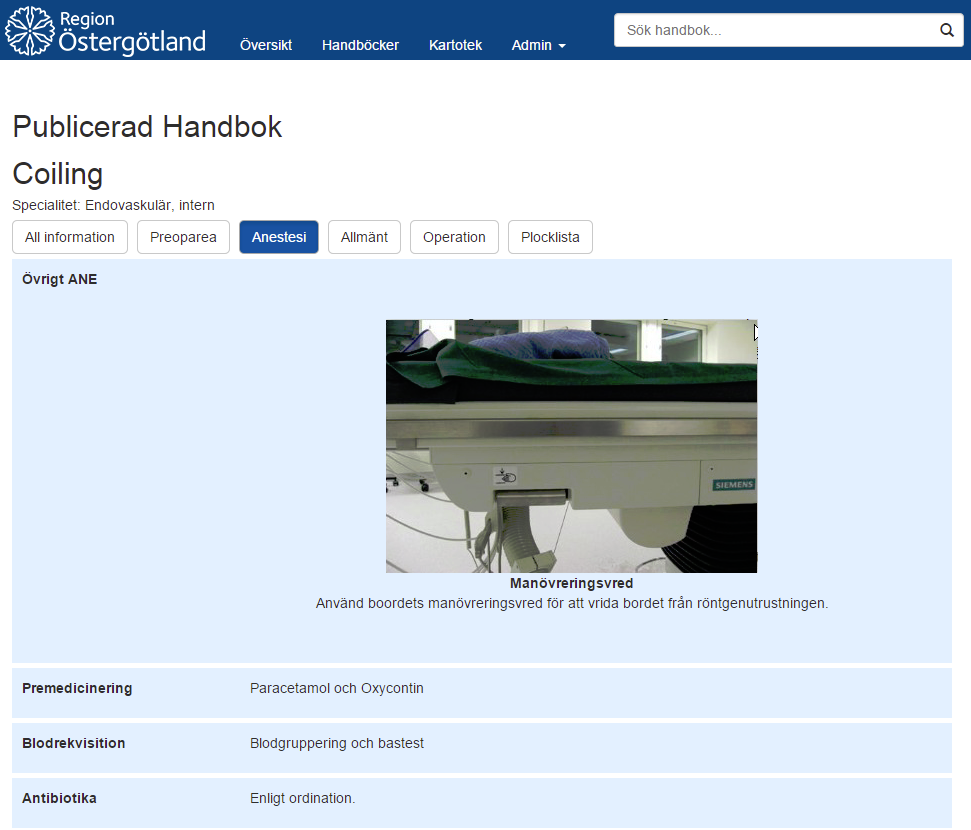
\includegraphics[scale=0.3]{handbok.png}
	\caption{Handböcker}
	\label{fig:handbok}
	\end{center}
\end{figure}

\begin{enumerate}
\item Filtrera handböckerna beroende på specialitet.
\item Filtrera handböckerna beroende på tillstånd.
\item Sök på handbok. Kan söka på namn eller alternativa sökord.
\end{enumerate}

Från adminmenyn kan man också lista handböcker under utkast och granskning direkt (se figur \ref{fig:adminmenyn}).

\begin{figure}[H]
	\begin{center}
	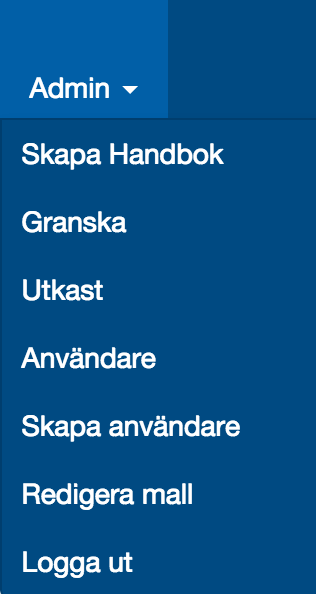
\includegraphics[scale=0.4]{adminmenyn.png}
	\caption{Adminmenyn}
	\label{fig:adminmenyn}
	\end{center}
\end{figure}

\section{Påbörja en förberedelse}
För att påbörja en förberedelse klickar man på ''Påbörja förberedelse'' i en publicerad handbok (se figur \ref{fig:paborja}). Man får då ange Linda-id (se figur \ref{fig:lindaid}).

\begin{figure}[H]
	\begin{center}
	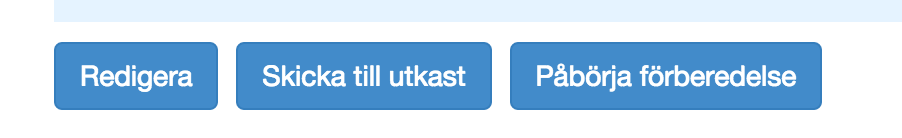
\includegraphics[scale=0.3]{paborja.png}
	\caption{Påbörja operationsförberedelse}
	\label{fig:paborja}
	\end{center}
\end{figure}

\begin{figure}[H]
	\begin{center}
	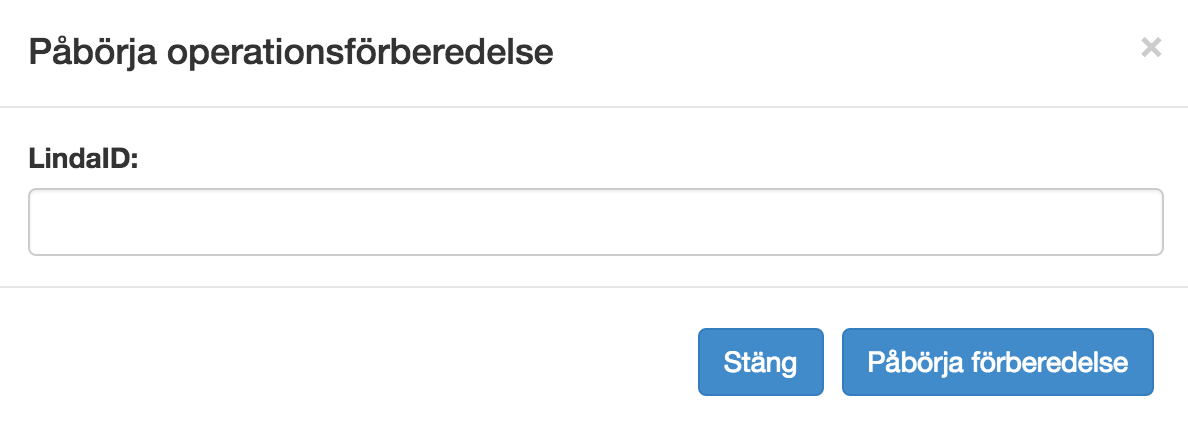
\includegraphics[scale=0.3]{lindaid.png}
	\caption{Ange Linda-id}
	\label{fig:lindaid}
	\end{center}
\end{figure}

\section{Redigera mall}
En mall för en ny handbok finns och kan redigeras. Denna redigering nås genom adminmenyn (Se figur \ref{fig:paborja}). Här kan man t.ex. lägga till vilka proccesssteg som ska finnas med som standard.

\begin{figure}[H]
	\begin{center}
	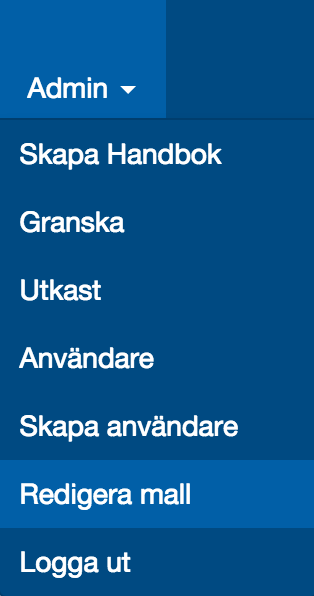
\includegraphics[scale=0.4]{redigeramall.png}
	\caption{Redigera mall}
	\label{fig:redigeramall}
	\end{center}
\end{figure}

\section{Användare}
Från adminmenyn kan man skapa nya och lista användare (se figur \ref{fig:adminmenyn2}). Man kan välja om en användare ska vara administratör. En användare som inte är administratör har samma rättigheter som en ej inloggad användare.

\begin{figure}[H]
	\begin{center}
	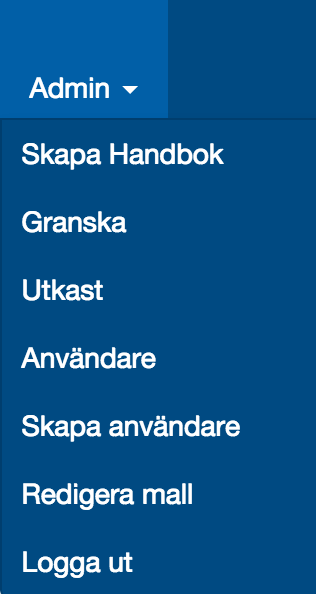
\includegraphics[scale=0.4]{adminmenyn2.png}
	\caption{Adminmenyn}
	\label{fig:adminmenyn2}
	\end{center}
\end{figure}

\end{document}